\documentclass{article}
\usepackage{luacode}
\usepackage{graphicx}
\graphicspath{ {data/} }
\begin{luacode*}
  function test()
    require("lualibs.lua")
    local file = io.open('data/data.json')
    local jsonstring = file:read('*a')
    file.close()
    local jsondata =  utilities.json.tolua(jsonstring)
    tex.print('\\begin{tabular}{cc}')
    tex.print('\\hline\\textbf{Scientific name} & \\textbf{Category} \\\\\\hline')
    for key, value in pairs(jsondata) do
      tex.print(value["scientific_name"] .. ' & ' .. value["category"] .. '\\\\')
      tex.print('\\\\')
    end
    tex.print('\\hline\\end{tabular}')
  end
\end{luacode*}
\begin{document}
\directlua{test()}
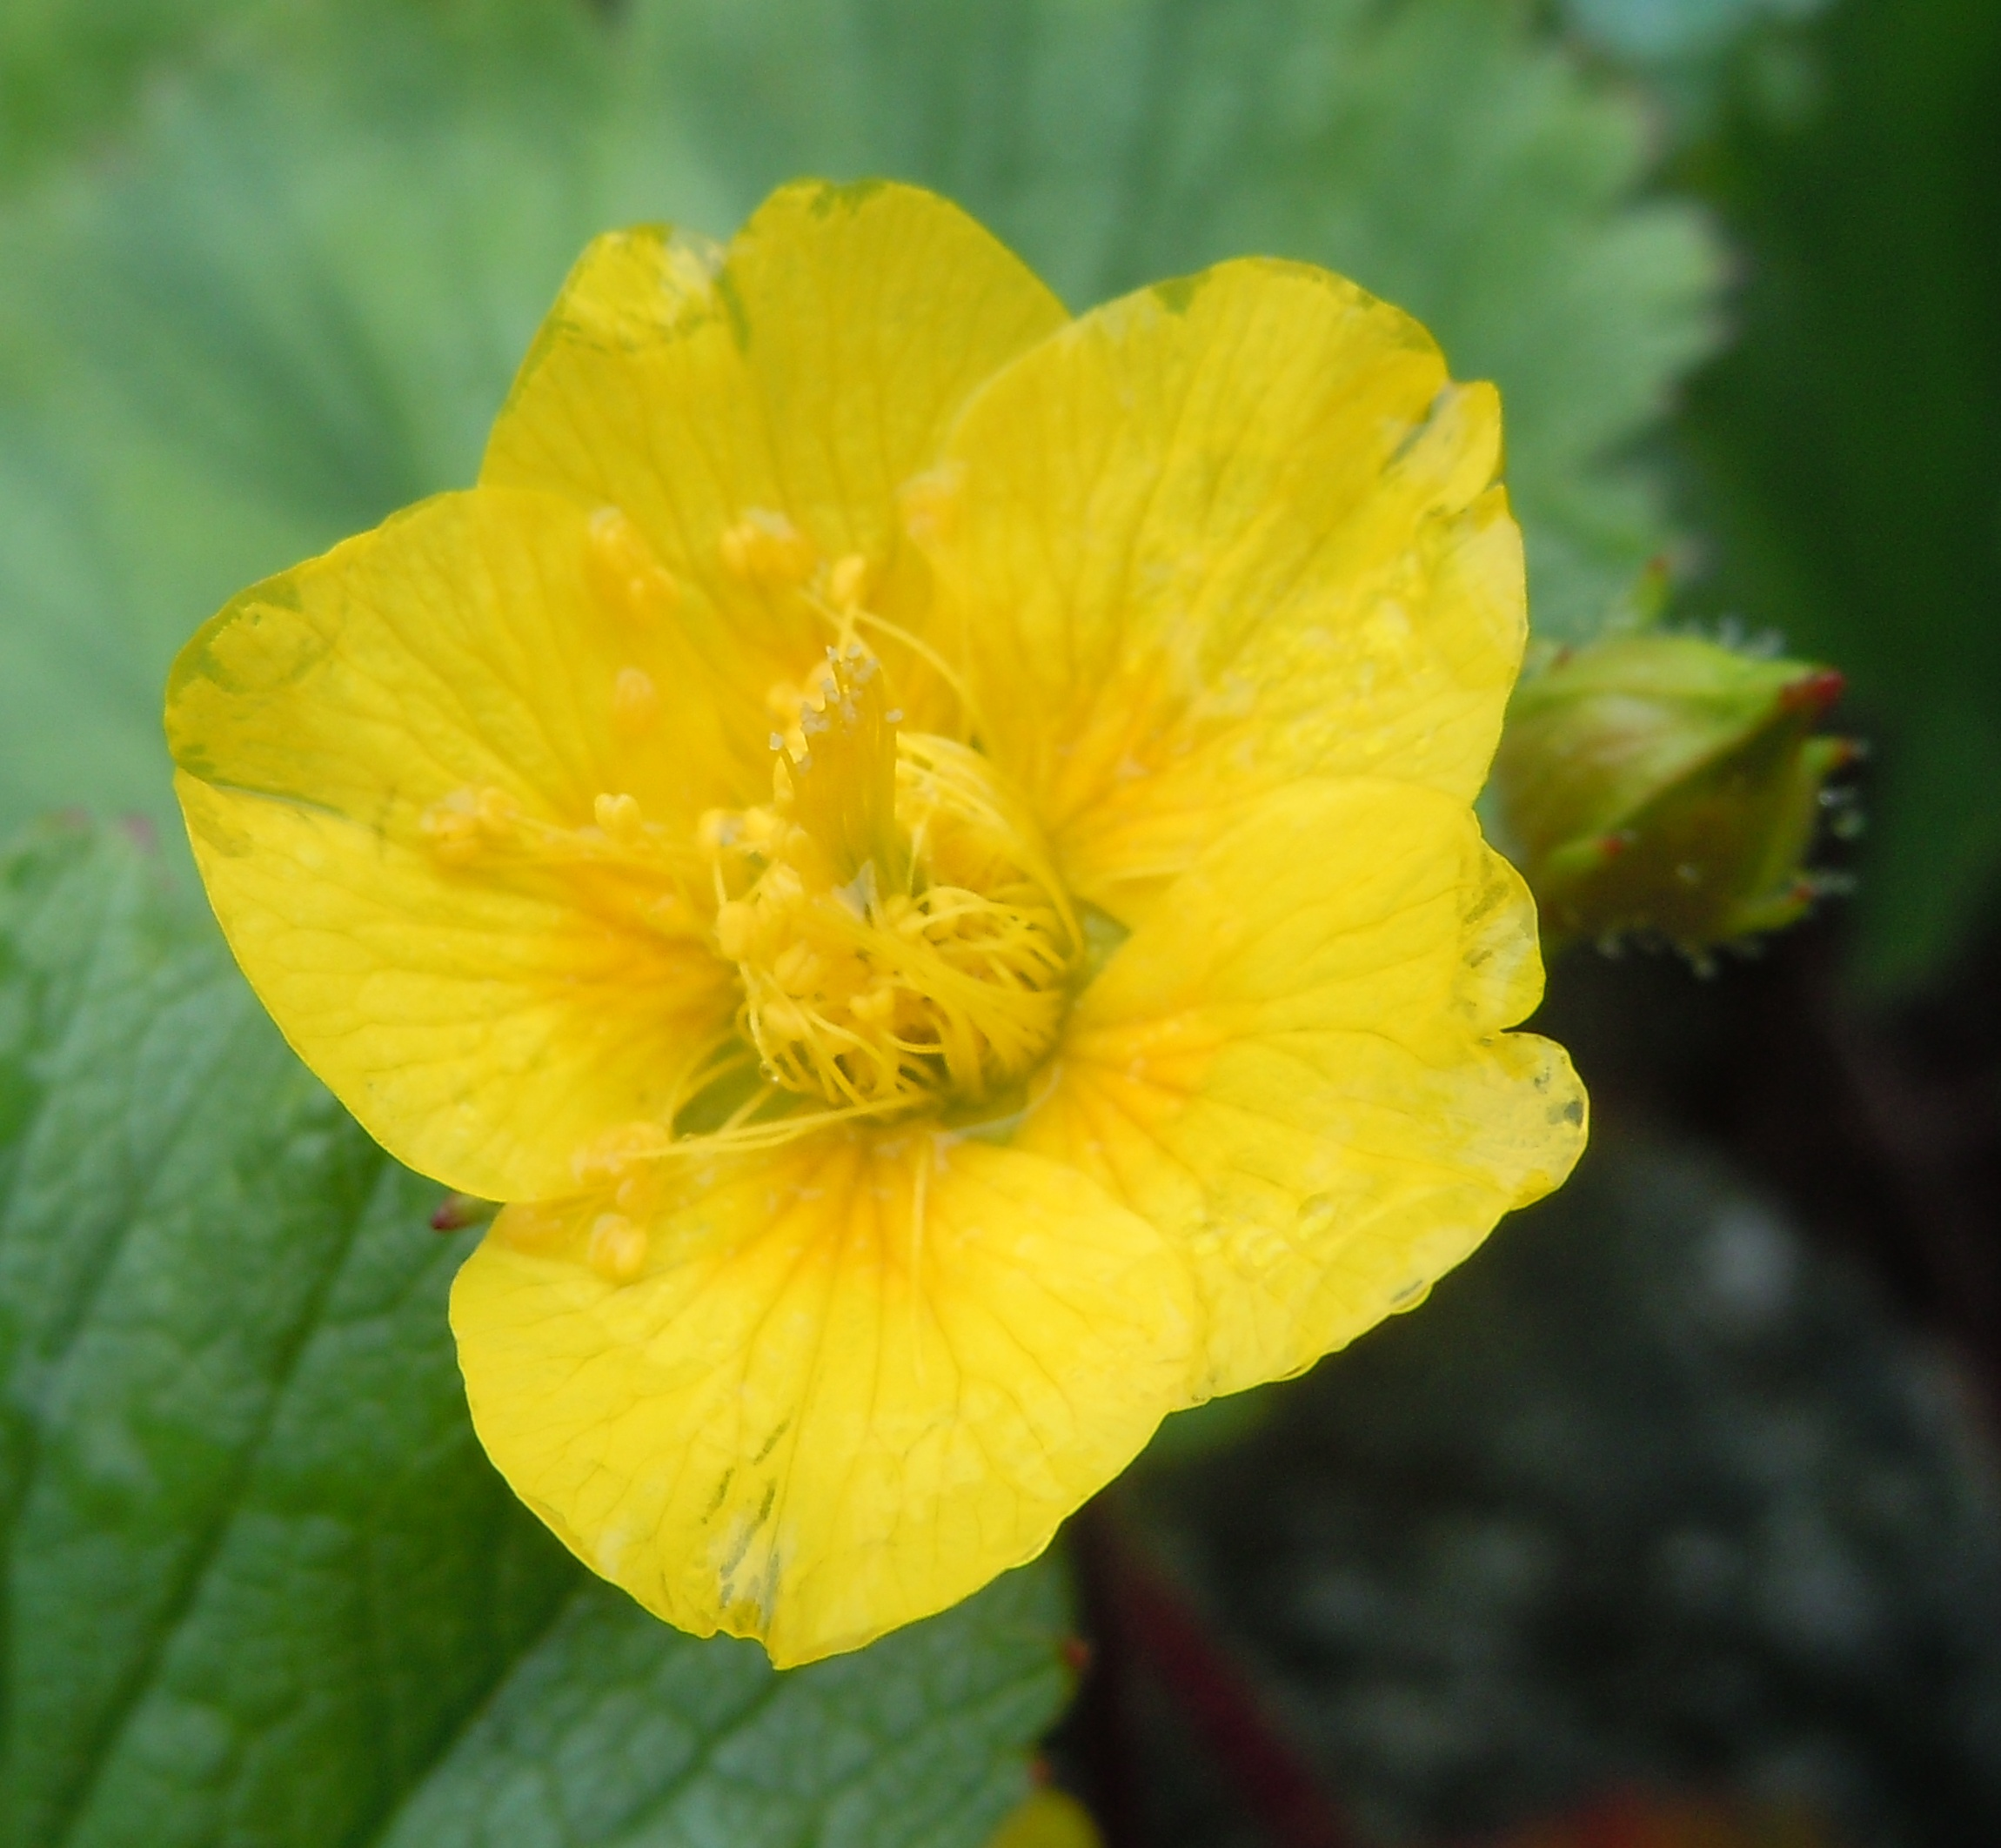
\includegraphics[width=5cm]{alpineflora/Geumpeckii}
\end{document}